\section{Coral reefs: a rich but threatened ecosystem}

Coral reefs are among the most productive and biologically diverse ecosystems on Earth \citep{connell1978diversity, moberg1999ecological}. They supply food, income and coastal protection to vast numbers of people (Fig. \ref{intro:corals}). While they account for less than 0.5\% of the ocean floor \citep{spalding1997new}, they are home for almost a third of the marine biodiversity \citep{moberg1999ecological}. Reef-related fisheries account to up to 40\% of the total marine
fish landed value of some regions \citep{teh2013global} and hundreds of millions of people depend on coral reefs for their livelihood or part of their protein intake \citep{salvat1992coral,hoegh2019people}. Through calcification, corals are the backbone of a complex three-dimensional habitat that serves as spawning, breeding and feeding area for many species \citep{moberg1999ecological}. This complex reef framework  dissipates most of incoming waves energy, protects shorelines from storms and floods, and prevents coastal erosion \citep{ferrario2014effectiveness,elliff2017coral}. Additionally, wave dissipation creates lagoon and sedimentary environment, providing favorable conditions for the growth of seagrass and mangrove ecosystems \citep{moberg1999ecological}.

\begin{figure}
    \centering
    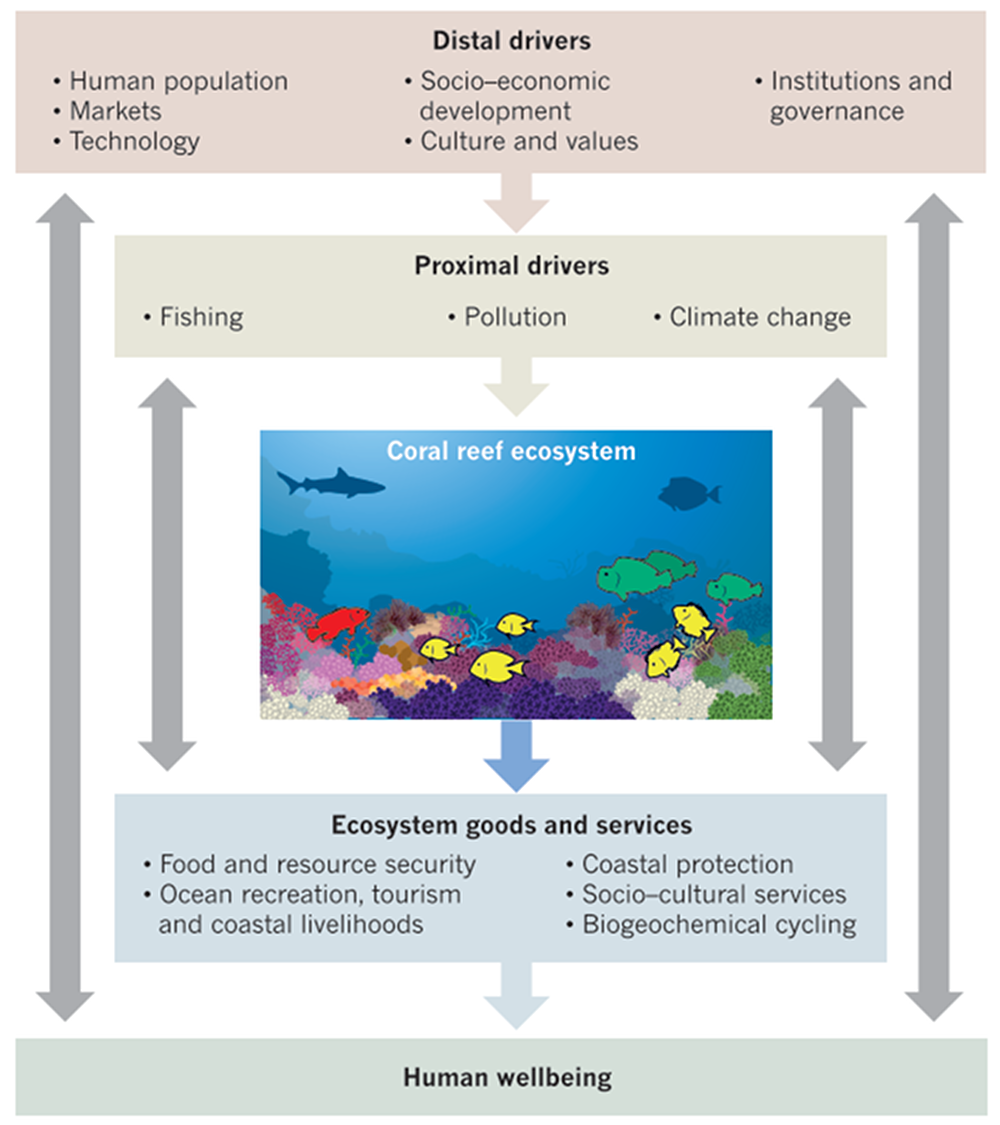
\includegraphics[width=.8\textwidth]{chapters/intro/figures/anthropocene.png}
    \caption{Goods and services of coral reefs and their linkage with human activities. Source: \cite{hughes2017coral}}
    \label{intro:corals}
\end{figure}

The calcifying process of reef building corals heavily depends on their symbiosis with the microalgae zooxanthellae. These unicellular symbionts convert sunlight and carbon dioxide into organic carbon and oxygen, providing the corals with most of the energy needed to meet their metabolic demands \citep{muscatine1977reef}. However, adverse environmental conditions such as elevated sea surface temperature can cause damage to the mechanisms maintaining this association, resulting in the expulsion of the endosymbionts \citep{hoegh2007coral}. This process, called bleaching, causes the coral to loose their pigmentation and reveals their underlying white skeleton \citep{baker2008climate}. Bleached corals are physiologically and nutritionally compromised, and prolonged bleaching over several months leads to high coral mortality \citep{hughes2018spatial}. Decline in coral health and cover pushes the reef ecosystem to a macroalgal-dominated state \citep{hughes2003climate,mumby2007thresholds}. Once a "tipping point" is exceeded, returning to a coral-dominated state becomes difficult \citep{mumby2007thresholds,graham2015predicting}.

Despite their importance, coral reefs have experienced a massive system-wide decline: it is estimated  that 50\% have already been severely damaged, and almost all could be lost under a 1.5$^\circ$C warming \citep{hoegh2019people,dixon2022future}. This global decline in live coral cover \citep{gardner2003long,pandolfi2003global,pandolfi2011projecting,bruno2007regional,perry2013caribbean,dove2020ocean} (Fig. \ref{intro:cover}) is caused by both global and local anthropogenic stressors. The main global stressors are climate change induced ocean warming and acidification. Ocean warming causes recurrent mass bleaching events at an increasing frequency \citep{connell199730, hughes2018spatial}. Furthermore, thermal stress can increase the susceptibility of corals to disease, leading to an increase in the incidence of coral disease outbreaks \citep{harvell2002climate,bruno2007thermal,muller2012caribbean}. Moreover, the increase of the concentration of atmospheric carbon dioxyde causes a decrease of the pH and carbonate concentration of seawater. As a result, coral calcification and growth decrease, which inhibits their capacity to build structurally complex habitats \citep{hoegh2007coral}. Local stressors are numerous and include pollution \citep{loya1980effects}, coastal development and the associated sediment and wastewater fluxes \citep{erftemeijer2012environmental, cunning2019extensive}, nutrient run-off \citep{hughes2003climate,sheppard2017biology}, and overfishing of herbivorous species controlling algae growth \citep{jackson2001historical}.

\begin{figure}
    \centering
    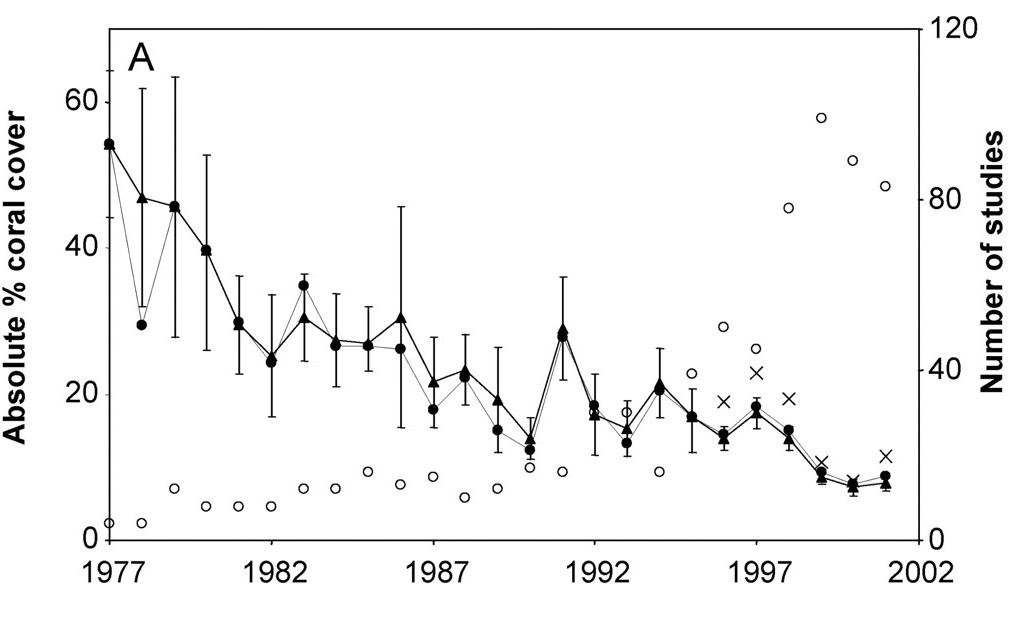
\includegraphics[width=.9\textwidth]{chapters/intro/figures/cover.jpeg}
    \caption{Evolution of the absolute coral cover in the Caribbean. Source: \cite{gardner2003long}}
    \label{intro:cover}
\end{figure}

Due to the combined damages from of all these stressors, it is almost impossible to return reefs to their past configurations \citep{hughes2017coral}. Instead, the challenge is now to maintain the biological functions of coral reefs through quickly changing environmental conditions. This will require to rapidly address greenhouse gas emissions, as well as local actions to boost the capacity of coral reef ecosystems to survive climate change \citep{hughes2003climate,knowlton2008shifting,graham2015predicting}. The aim of the present dissertation was therefore to use modeling tools to better understand the drivers of coral demise and hence inform such local actions to support ecosystem management in Florida, the third largest barrier reef of the world.

\section{Identifying the threats to coral survival in Florida}

The Florida Reef Tract (FRT) spans over approximately 577 km from the Dry Tortugas (DRTO) west of the Florida Keys to the St. Lucie Inlet in Martin County, constituting the third largest barrier reef in the world \citep{finkl2008shelf} (Fig. \ref{intro:frt}). These reefs harbor a rich Caribbean fauna, including more than 40 species of stony corals \citep{banks2008reef,jackson2014status}. The northern half-section of the FRT consists of relic, Holocene framework reefs and indurated sand ridges, divided into three shore-parallel reefs (inner, middle, outer) separated by sandy plains. Benthic cover is generally denser on the middle and outer reefs while the inner reef harbors some large patches of dense \textit{Acropora cervicornis}. The dominant reef builder is the bouldering \textit{Montastraea cavernosa} but living hard coral cover is fairly low (below 3\%)\citep{banks2008reef,walton2018impacts}. The southern half-section is a chain of limestone islands (the Keys) that extend from the southern tip of the Florida mainland southwest to the DRTO on the the boundary of the West Florida Shelf (WFS). The Upper Keys are remnants of ancient coral reefs and the Lower Keys are sand bars \citep{hoffmeister1968geology}. The DRTO are made of small circular reef banks whose coral populations are among the most preserved of the continental United States \citep{hine2008coral, kourafalou2018physical}. Moreover, they are believed to be important sources of recruitment for coral-reef fishes in the Florida Keys \citep{domeier2004potential}. 

\begin{figure}
    \centering
    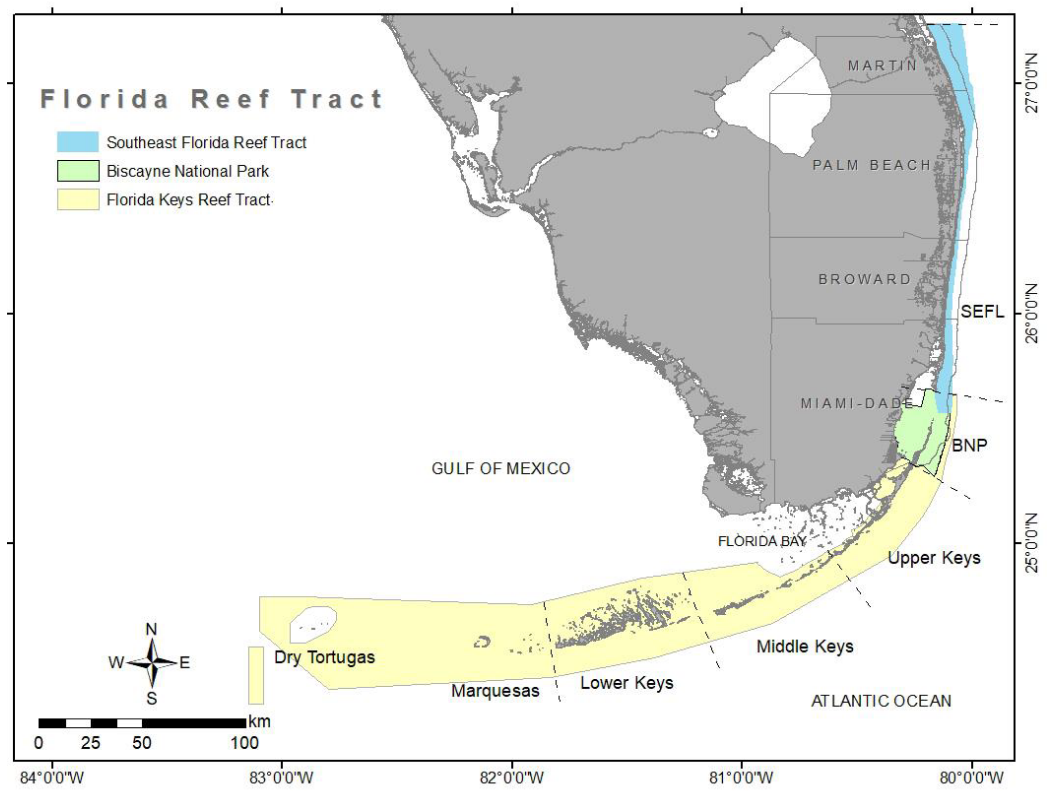
\includegraphics[width=\textwidth]{chapters/intro/figures/frt.png}
    \caption{Map of Florida Reef Tract with major features and divisions. Source: \cite{kupfner2019untapped}}
    \label{intro:frt}
\end{figure}

Florida's Coral Reef (FCR) is of considerable importance to the economy of the state. \cite{johns2003socio} estimated the contribution of recreational users of natural and artificial reefs over the period June 2000 to May 2001 to have been US\$2.3 billions in sales and US\$1.1 billion in income. Moreover, recreational use of the reefs was evaluated to bring 36,500 full and part-time jobs. Focusing on natural reefs only, \cite{brander2013total} estimated the total coral reef values Florida to be US\$174 millions. However, this value might be strongly underestimated as non-use and indirect use values, such as support for coastal fisheries \citep{ault2006building} and coastal protection \citep{ferrario2014effectiveness} were not taken into account.

Nevertheless, FCR has been heavily impacted by the human activities of the major metropolitan area of greater Miami. These impacts include densely populated coastlines, large numbers of visitors, polluted terrestrial run-off and overfishing \citep{jackson2014status}. For example, dredging operations during the PortMiami Deep Dredge Project (PMDDP) was reported to have caused the death of $>$560,000 corals \citep{cunning2019extensive}. Florida's coral reefs have therefore declined significantly over the past decades due to anthropogenic stressors and numerous disease outbreaks \citep{gardner2003long, jackson2014status}. Populations of previously dominant reef-building acroporids almost totally disappeared throughout the Caribbean and Florida \citep{aronson2001white}, and coral cover dropped from 40 to 60\% in 1975 to $<$7\% in the Florida Keys \citep{jackson2014status} and $<$3\% in the northern section of the FRT \citep{walton2018impacts}. Furthermore, since 2014, many coral species have experienced widespread and severe decline caused by the ongoing outbreak of stony coral tissue loss disease (SCTLD). For instance, populations of \textit{M. cavernosa}, once one of the most abundant species of the FRT, decreased by 45\% in abundance between 2015 and 2016 \citep{walton2018impacts}.

Coral disease outbreaks are frequent in the Caribbean, which is considered as a disease "hot spot" because of the fast emergence, high prevalence, wide geographic distribution, and virulence of coral diseases in the area \citep{green2000significance, harvell2007coral}. For instance, populations of  \textit{Acropora} spp. decreased by $>$95\% throughout the Caribbean during numerous outbreaks of white-band disease in the 1970-1990s \citep{aronson2001white}. Other major outbreaks include the white plague and black band diseases, that respectively affect 22 and 42 corals species and caused significant declines in reef-building coral populations in the Caribbean \citep{bruckner2003field,miller2009coral, muller2011black}. 

The latest major outbreak affecting coral reefs of the Caribbean is the SCTLD \citep{noaa2018}. First observed off the coasts of Miami in 2014 during the PMDDP \citep{precht2016unprecedented}, the disease has since spread throughout the entire Florida Reef Tract and numerous territories of the Caribbean \citep{alvarez2019rapid, kramer2019map, estrada2021effects} (Fig. \ref{intro:propagation}). The outbreak affects at least 24 species of scleractinian coral and often results in whole colony mortality \citep{precht2016unprecedented, walton2018impacts}. Briefly, the gross morphology of SCTLD can be focal or multifocal, with locally extensive to diffuse areas of acute to subacute tissue loss distributed basally, peripherally, or both. In some cases, tissues bordering areas of chronic tissue loss show indistinct bands of pallor, progressing to normal pigmentation away from the denuded skeleton (Fig. \ref{intro:sctld}). The continued persistence of the outbreak, the high number of species affected, and its large geographical distribution suggest that SCTLD might be the largest coral disease outbreak on record in Florida. Although the causative agent of the disease remains unknown, there is evidence of waterborne disease transmission \citep{aeby2019pathogenesis,eaton2021measuring,meiling2021variable} and recent studies showed evidence that sediments can act as a vector for the SCTLD \citep{rosales2020rhodobacterales, studivan2022reef}. 

\begin{figure}
    \centering
    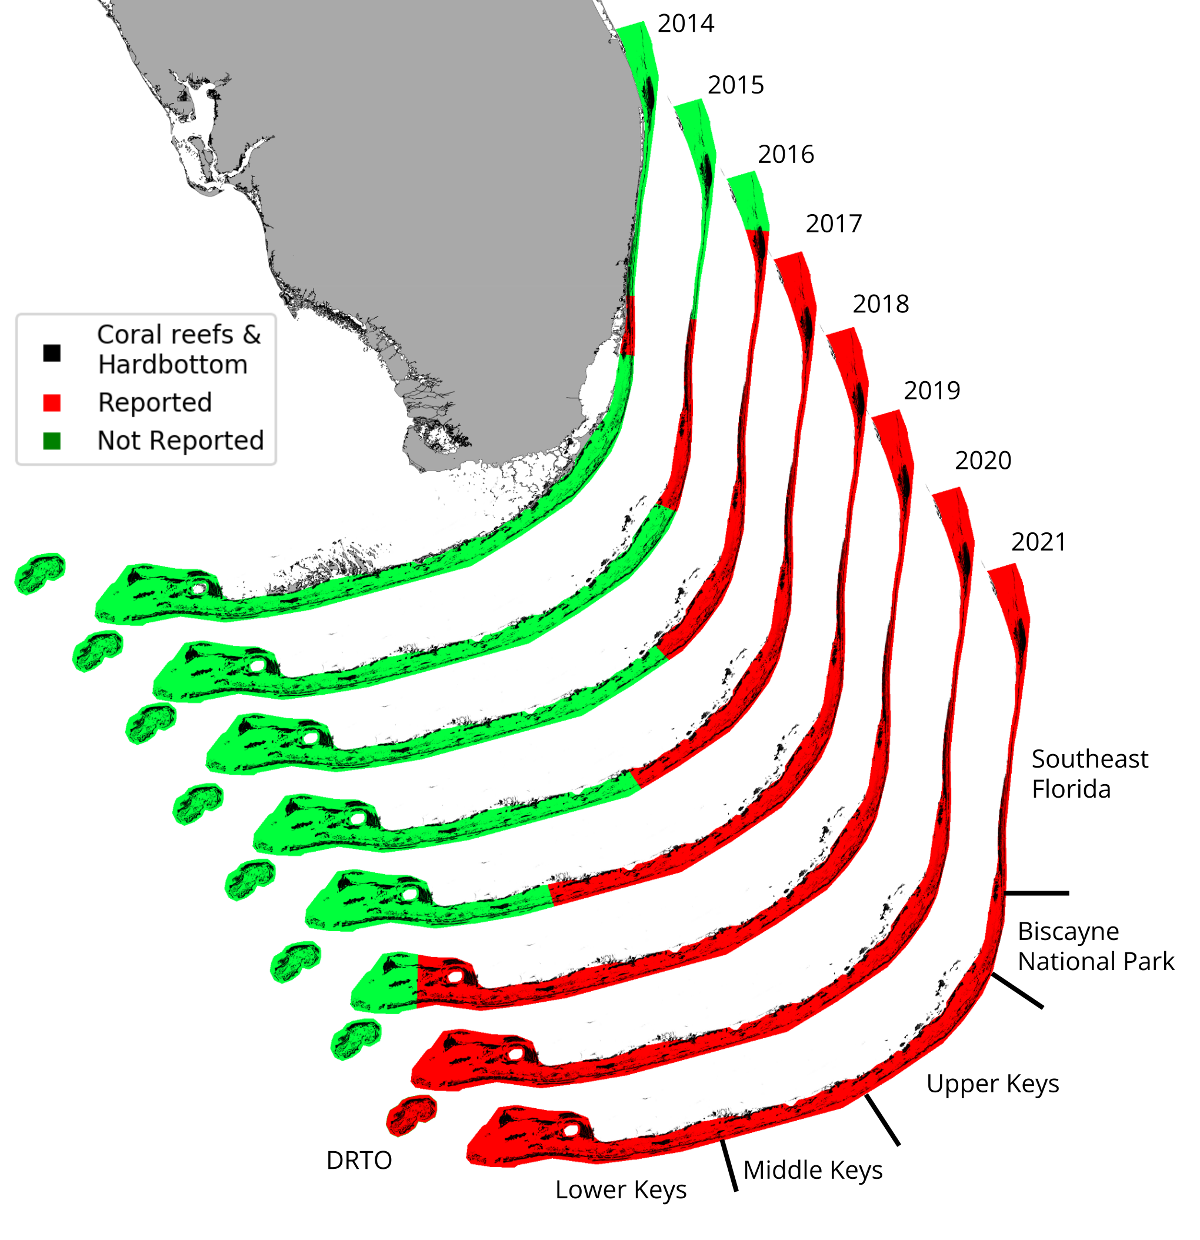
\includegraphics[width=\textwidth]{chapters/intro/figures/fig_sctld.png}
    \caption{Propagation of the SCTLD troughout the FRT between 2014 and 2021}
    \label{intro:propagation}
\end{figure}

\begin{figure}
    \centering
    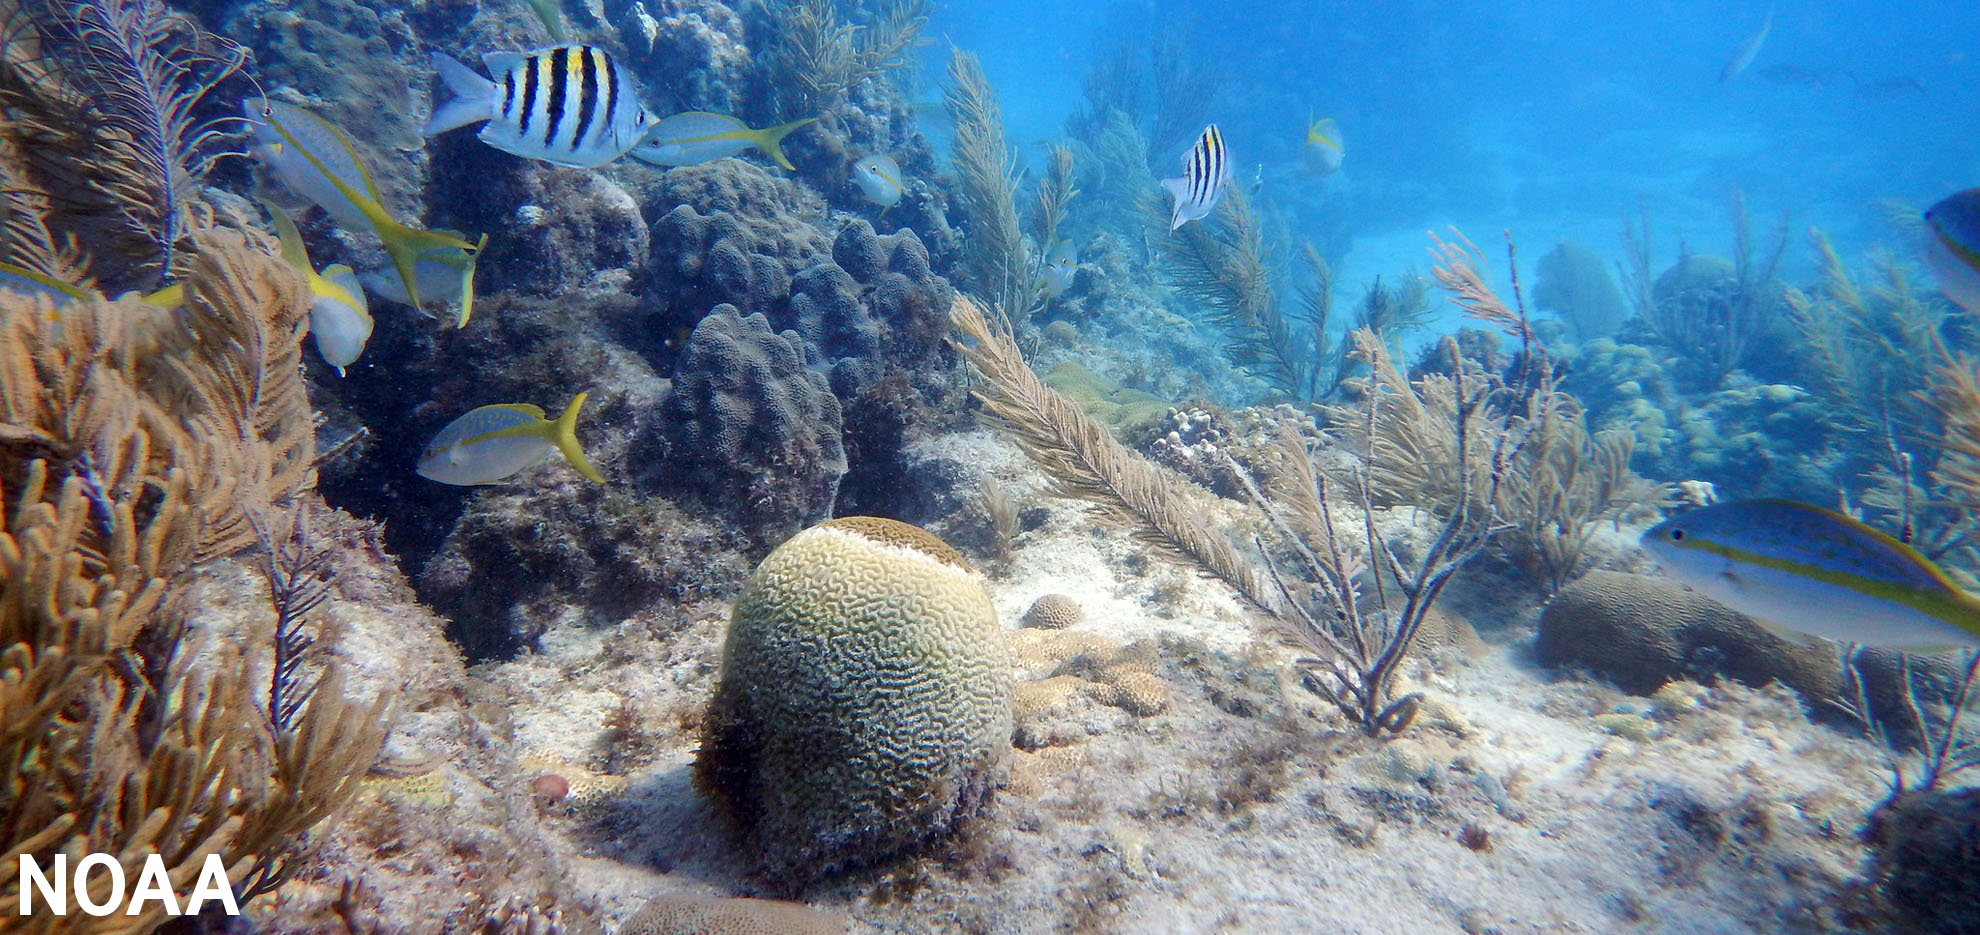
\includegraphics[width=\textwidth]{chapters/intro/figures/sctld.jpg}
    \caption{Brain coral affected by SCTLD in Looe Key, Florida. The disease is leaving a white band of recently dead skeleton in contrast to the healthy, yellow/brown tissue. Source: Florida Fish and Wildlife Research Institute}
    \label{intro:sctld}
\end{figure}

Additionally, Florida is a prime landfall target for tropical cyclones from June through November (Fig. \ref{inro:landfall}). Between 1899 and 1998, Southeastern Florida has been directly hit by 27 hurricanes, 5 of which were of category 4 or more (winds $>$ 209 km/h) \citep{neumann1999tropical}. Hurricanes that forms in June and July are usually weak while hurricanes occurring in August and September tend to become severe storms \citep{banks2008reef}. This is illustrated by Hurricane Irma, one of the strongest and costliest hurricanes on record in the Atlantic, that made landfall in Florida in September 2017 as a category 4 hurricane \citep{irmaNOAA, xian2018brief}. Hurricanes are a major agent of coral mortality in the Caribbean that contributed to the decline of acroporids \citep{gardner2003long,gardner2005hurricanes,aronson2001white}. They cause a wholesale destruction of the reef biota on their passage and can induce coral burial through sediment resuspension \citep{banks2008reef, miller2008effects, tweel2014contribution}. Furthermore, they significantly impact the content of surface waters through upwelling and mixing, which can disturb the benthic communities \citep{wachnicka2019hurricane,varlas2020investigating}. Moreover, heavy wind conditions generate important waves that interact with currents and significantly alter transport processes in nearshore waters \citep{niu2017role,mao2020particle}. This might impact the dispersion of coral larvae, that are released during the hurricane season \citep{hendee1998champ}. Hurricane might therefore interrupt larval exchanges between otherwise connected reefs but also create new connectivity pathways. As major hurricanes are intensifying under the effect global warming \citep{bhatia2019recent,knutson2020tropical}, better understanding the impact of hurricanes on wave-induced processes could inform the management of reefs under future climatic conditions. Furthermore, as incoming storm-generated waves dissipate over reefs, better understanding the protective role of coral reefs might promote their restoration as tool to reduce coastal flooding hazard \citep{roelvink2021coral}.

\begin{figure}
    \centering
    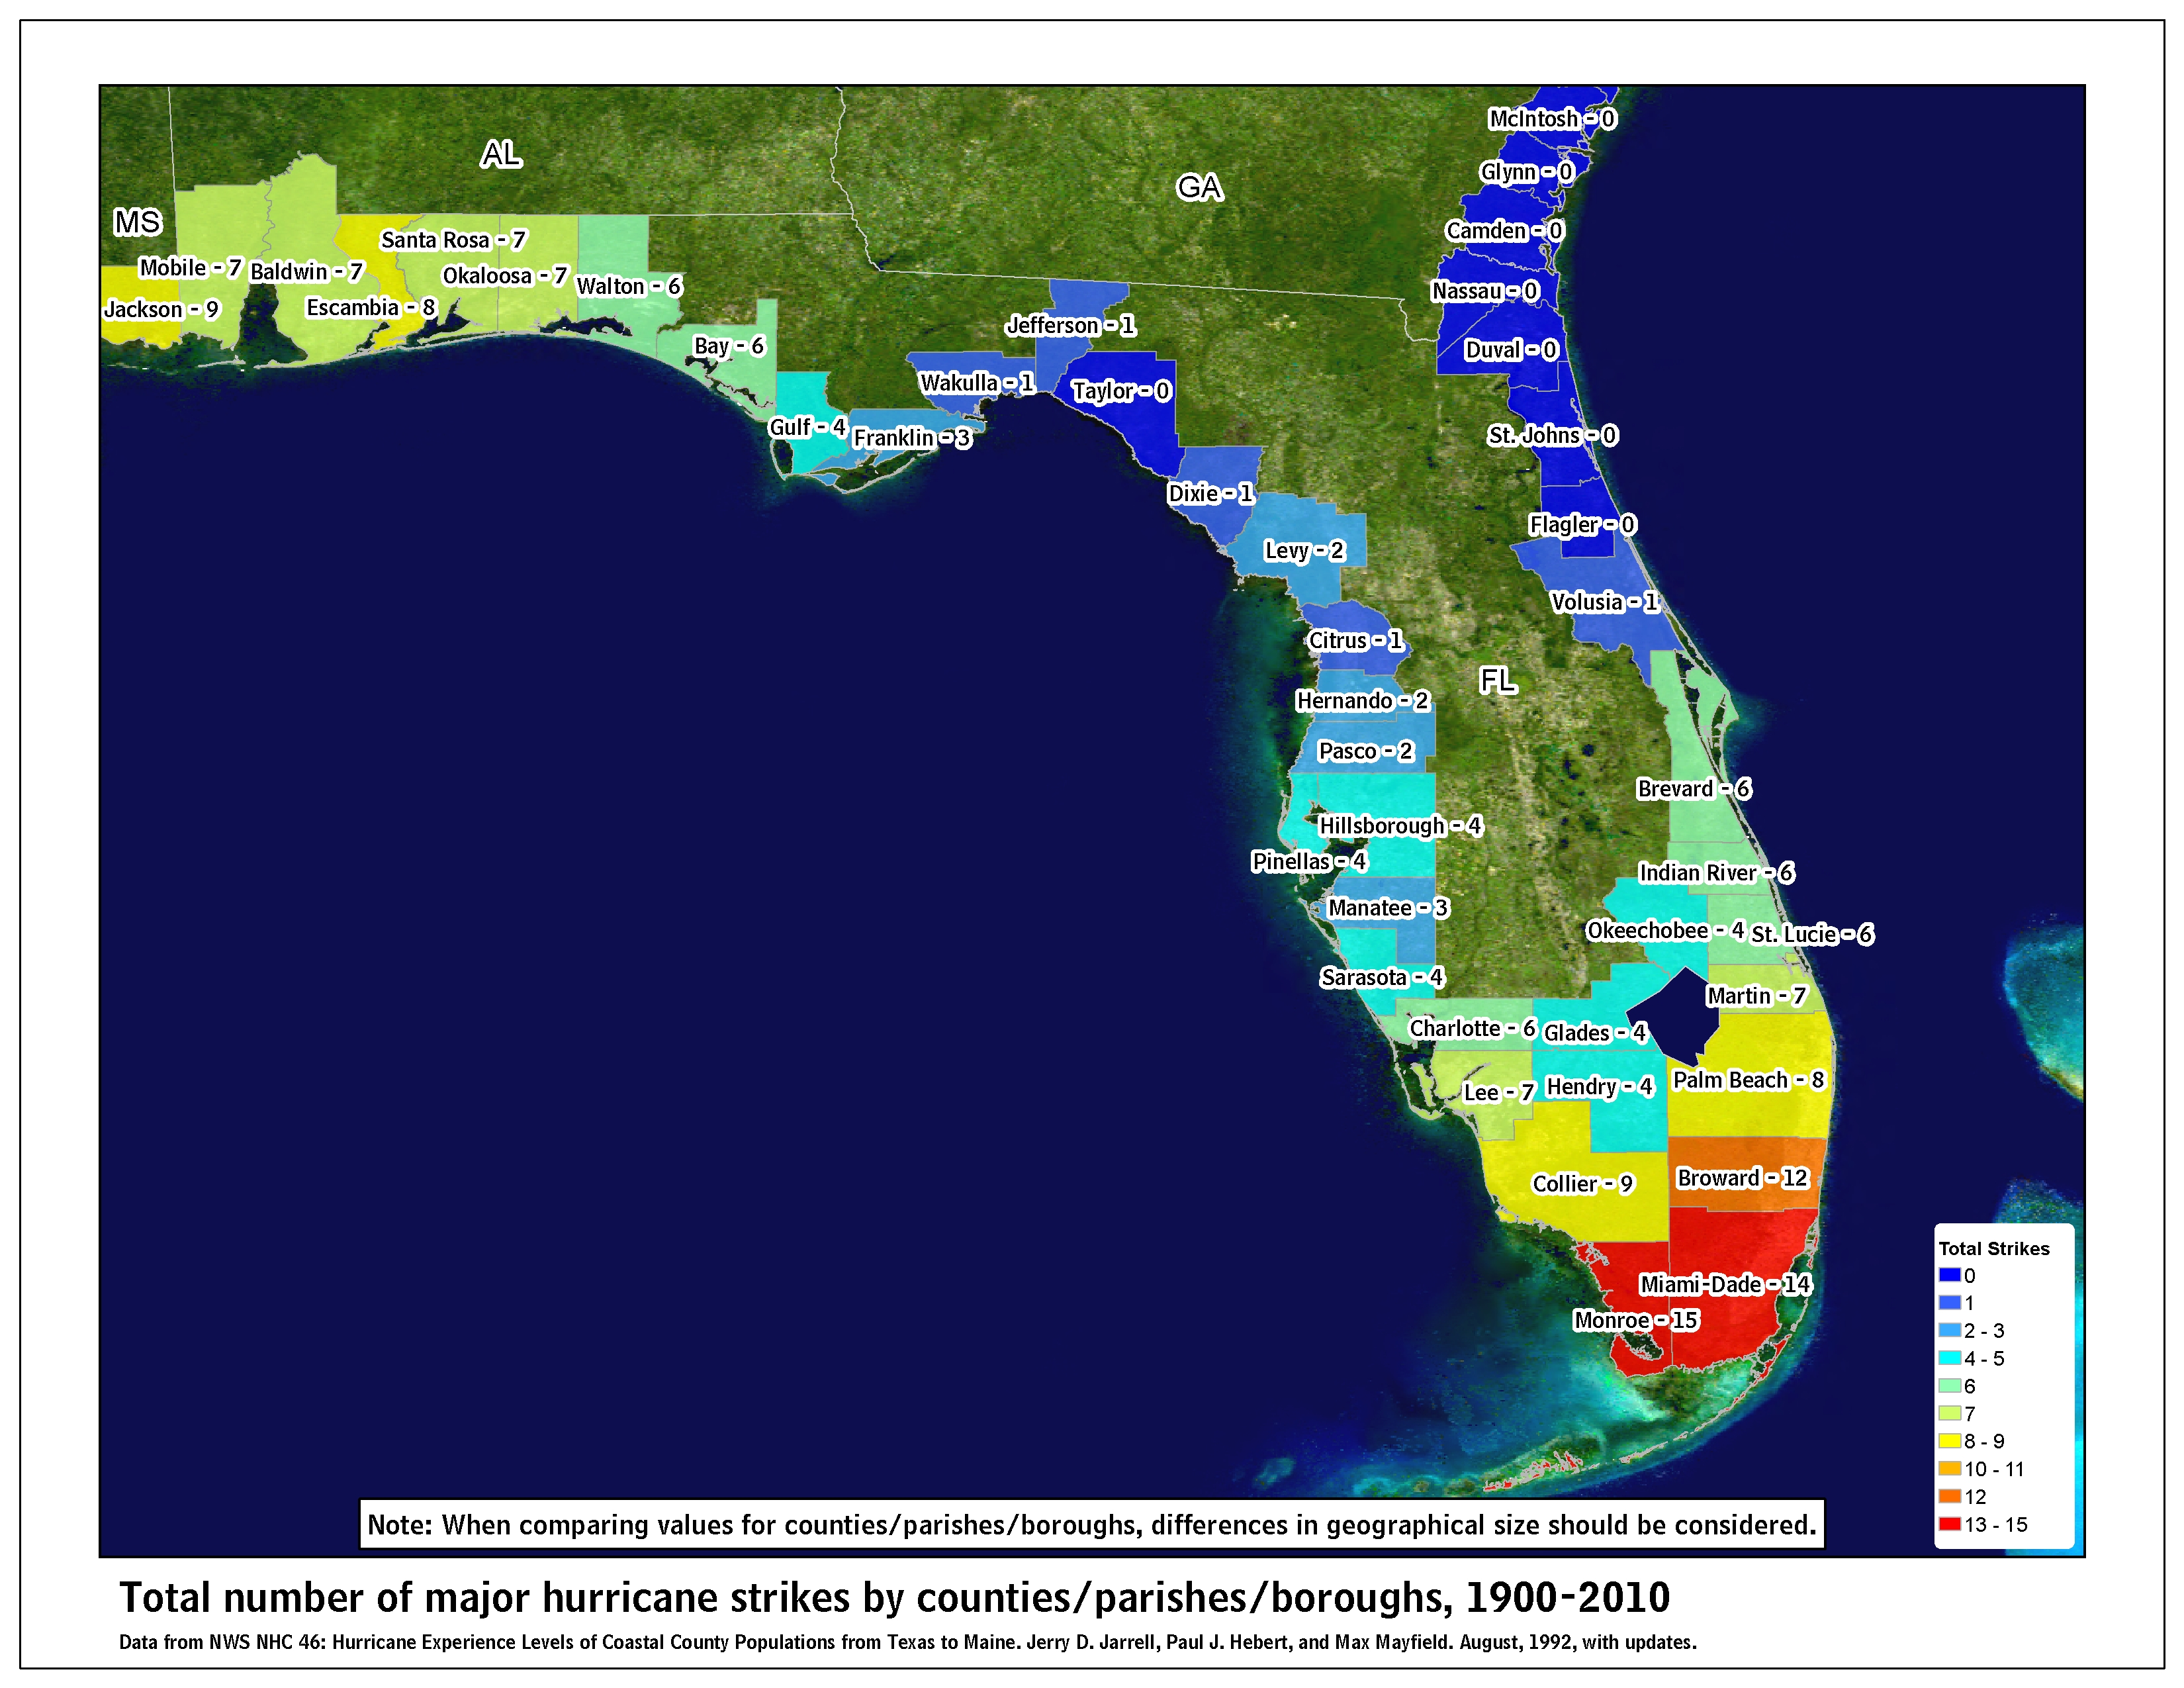
\includegraphics[width=\textwidth]{chapters/intro/figures/hurricane_strikes.jpg}
    \caption{Total number of major hurricanes strikes in Florida between 1900-2010. Source: National Oceanographic and Atmospheric Administration, National Hurricane Center \url{https://www.nhc.noaa.gov/climo/}}
    \label{inro:landfall}
\end{figure}

\section{Thesis objectives}

This thesis focuses on two main threats that could jeopardize the future and survival of FCR: the current outbreak of SCTLD and hurricanes. These threats were studied by fulfilling four main objectives. First, as SCTLD was expected to propagate through waterborne transmission, we developed a coupled epidemio-hydrodynamic model to reproduce the observed spread of the outbreak through the FRT. Such a model provides novel insight into the management of the epidemic, the identification of its causative agent, and its mode of transmission. Second, we used this model to explain the timing of the propagation of SCTLD within the FRT. More specifically, we investigated whether the modeled hydrodynamics were explanatory of the apparent stalling of the outbreak between the Marquesas and the DRTO in 2020. Third, as sediments can act as vector for the disease, we evaluated the impact of the PMDDP on the reported onset of SCTLD in 2014 using a sediment transport model. We assessed whether sediments produced or resuspended during dredging operations might have been transported to reefs where disease was reported and evaluated whether the timing of these sediment fluxes was consistent with the observed spread of the disease. Finally, we developed a coupled wave-current model to evaluate the impact of hurricanes on wave-induced transport processes. This model was applied to Irma, a major hurricane that made landfall in the Florida Keys in 2017, during the reproduction period of several coral species.

These objectives can be summarized into four main questions:
\begin{enumerate}
    \item How did the SCTLD spread through the FRT ?
    \item What caused the apparent stalling of the propagation of SCTLD ? 
    \item What was the impact of the PMDDP on the onset of the oubreak of SCTLD~?
    \item  What is the effect of hurricane-induced wave-current interactions on transport processes and should they be taken into account when modeling the dispersal of coral larvae ?
\end{enumerate}     
Answering these four questions required the use of an ocean model able to capture both the large-scale ocean features influencing circulation along the FRT as well as small-scale flow features down to the reef scale. A description of the main hydrodynamic features of the FRT as well as an overview of the modeling tools used in this thesis are given in the next section.

\section{Modeling hydrodynamics and transport processes in the FRT}
The FRT is located along the northern side of the Straits of Florida, that connects the Gulf of Mexico (GoM) and the North Atlantic Ocean. The large-scale circulation in this region is dominated by the interplay of the Florida Current (FC) and the Loop Current (LC). The LC is an area of warm waters from the Caribbean Sea that enters the GoM through the Yucatan Channel and then loops anti-cyclonically through the northeastern Gulf of Mexico and finally exits through the southern Straits of Florida, where it forms the Florida Current (FC). The FC then flows northward between Florida and the Great Bahama Bank to form the Gulf Stream (Fig. \ref{intro:gom}). The northward penetration of the LC through the GoM varies throughout the year, and sporadically an anticyclonic ring separates from the current \citep{leipper1970sequence, maul1977annual, vukovich1988loop}. The detachment of these anticyclonic eddies from the main LC affects in turn the position of the FC, causing its meandering along the FRT. These variations of the FC position have been shown to have no seasonal pattern with strong interannual variability. The generated meandering is associated with the presence of cyclonic eddies between the core of the current and the FRT \citep{kourafalou2012florida}. These eddies significantly impact the ecology of the southwest Florida Shelf by causing larval retention on the shelf and delivering larval pulses to the Upper Keys \citep{lee1994evolution, sponaugle2005florida, kourafalou2012florida}. Furthermore, when the LC meets the shallow waters of the southwest corner of the WFS near the DRTO, it causes the inflow of nutrients that modify water properties on the shelf \citep{weisberg2003local, liu2016offshore}. These contacts have been hypothesized to impact in turn the penetration of the LC in the GoM \citep{weisberg2017loop}. However, on the northernmost section of the FRT, eddies generated by the meandering of the FC cause cold-water upwelling limiting the northern range of tropical species \citep{walker2013determining}. The circulation on the upper part of the shelf along the FRT is largely influenced by winds, as well as diurnal and semi-diurnal tidal processes \citep{lee2001transport, lee2002volume,d2007patterns}

\begin{figure}
	\centering
	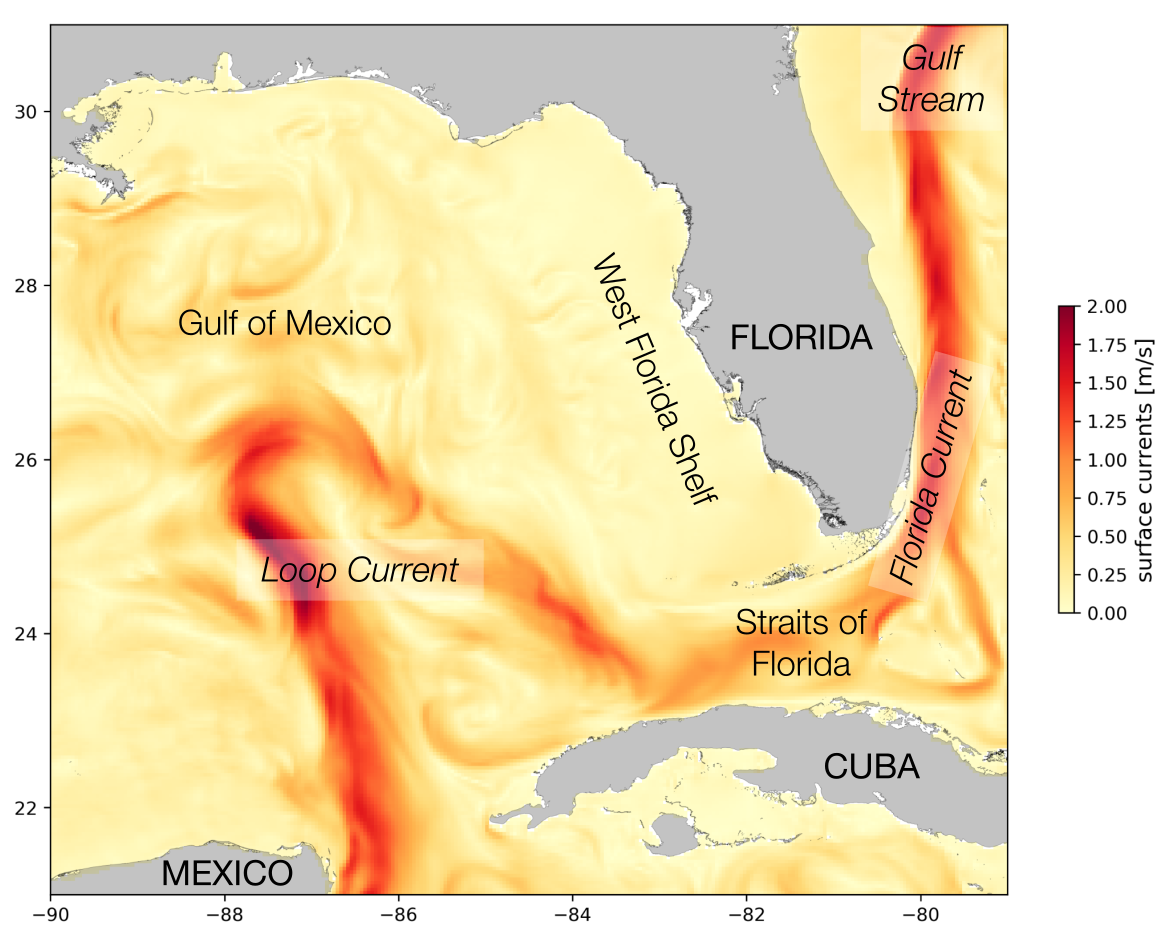
\includegraphics[width=.9\textwidth]{chapters/intro/figures/fig_gom.png}
	\caption{An example of the Loop Current and the Florida Current on January 12, 2019 as shown by HYCOM.}
	\label{intro:gom}
\end{figure}

The aforementioned large-scale ocean circulation significantly impact transport processes in the FRT. The modeling tools developed in this thesis should therefore be able to capture them accurately. Furthermore, as our objective is to model the dispersal of disease agents and sediments in a topologically complex coastal reef ecosystem, our modeling framework should also be able to capture small-scale ocean circulation features. For instance, small-scale flow features such as recirculation eddies around reefs and islands have been shown to strongly influence larval dispersal by increasing their local retention over the reefs \citep{figueiredo2013synthesizing}. Furthermore, accurately capturing the topography of coastal areas is critical when modeling storm conditions, as large wind waves generate strong currents, waves and storm surges in nearshore regions \citep{dietrich2010high, weisberg2006hurricane}. Unstructured-mesh models offer a well-suited solution to capture the multi-scale nature of flow features in the FRT in a computationally tractable way. They allow to locally refine the model resolution to $\sim~100$ m close to reefs and island while covering a domain large enough to capture the impact of the FC \citep{lambrechts2008multi,frys2020fine}. In contrast, the best resolution currently available in the Florida Keys using structured-grid models is $\sim900$ m (FKeyS-HYCOM, \citealp{kourafalou2012florida}). Nested grid models are another possible approach \citep{warner2010development} but they lack the flexibility required to adapt to the complex topology of coastal regions \citep{fringer2019future}.

In this thesis, we used the 2D barotropic version of the unstructured-mesh Second-generation Louvain-la-Neuve Ice-ocean Model (\href{https://www.slim-ocean.be/}{SLIM}). This model relies on Discontinuous Galerkin finite element methods \citep{aizinger2002discontinuous} and has already been successfully used to model the hydrodynamics of the whole Great Barrier Reef \citep{lambrechts2008multi}. Moreover, by coupling SLIM with the HYbrid Coordinate Ocean Model (HYCOM-GOMl0.04, \citealp{chassignet2007hycom}), SLIM was able to indirectly represent the baroclinic dynamics of the FC. Using this coupling, \cite{frys2020fine} successfully modeled coral larval connectivity in the FRT, \ie~the exchanges of larvae between reefs. In this study, coral larvae were modeled using a Lagrangian particle tracking model forced by SLIM currents. To answer our different research questions, we adapted this larval transport model to evaluate the dispersal of the causative agent of the SCTLD and sediments particles.

At the beginning of this thesis, SLIM was not able to represent wave-current interactions under storm conditions. Heavy winds generate large wind-waves that disturb ocean conditions and interact non-linearly with the currents \citep{liu2020impacts,wu2011fvcom}. The wave-generated currents cause water level variations near shorelines and wave breaking points which, in turn, affect the motion and evolution of the waves \citep{longuet1970longshore, sikiric2013coupling}. Capturing wave-current interactions hence requires the calculation of the full directional wave spectrum in order to correctly reproduce the dynamics of wind-driven surface waves. This is usually achieved by spectral wave models, which describe the evolution of the wave energy spectrum. An objective of this thesis was therefore the coupling of SLIM with the spectral wave model Simulating WAve Nearshore (SWAN, \citealp{booij1999third}), specifically developed for coastal applications and relies on numerical schemes adapted to small-scale, shallow water regions. Further details on the models and their coupling is given in chapter \ref{chap:irma}.

\section*{Outline}
This thesis is mainly a collection of publications describing our answers to the four main research questions. Chapter \ref{chap:sctld} describes the development of a coupled epidemio-hydrodynamic model to reproduce the observed spread of SCTLD in the FRT. Chapter \ref{chap:drto} explains how this model was used to study the apparent stalling of the spread of the SCTLD between the Marquesas and the DRTO. Chapter \ref{chap:onset} investigates the impact of the PMDDP on the onset of the SCTLD oubreak in 2014. Chapter \ref{chap:irma} describes the development of a coupled wave-current model to study the impacts of Hurricane Irma (2017) on wave-induced transport processes in the Florida Keys. Finally, chapter \ref{chap:conclusion} presents the conclusions of this thesis and perspectives for further works. 

\newpage
\section*{Supporting publications}

\begin{list}{}{%
    \setlength{\topsep}{0pt}%
    \setlength{\leftmargin}{0.23in}%
    \setlength{\listparindent}{-0.23in}%
    \setlength{\itemindent}{-0.23in}%
    \setlength{\parsep}{\parskip}%
    }%
        
    \item \textbf{Dobbelaere, T.}, Muller, E. M., Gramer, L. J., Holstein, D. M., \& Hanert, E.
    (2020). Coupled epidemio-hydrodynamic modeling to understand the spread
    of a deadly coral disease in Florida. \textit{Frontiers in Marine Science}, 7, 1016. \href{https://www.frontiersin.org/articles/10.3389/fmars.2020.591881/full}{doi: 10.3389/fmars.2020.591881}
    
    \item \textbf{Dobbelaere, T.}, Curcic, M., Le Hénaff, M., \& Hanert, E. (2022). Impacts of Hurricane Irma (2017) on wave-induced ocean transport processes. \textit{Ocean Modelling}, 101947. \href{https://www.sciencedirect.com/science/article/pii/S1463500322000026}{doi: 10.1016/j.ocemod.2022.101947}
    
    \item \textbf{Dobbelaere, T.}, Holstein, D. M., Muller, E. M., Gramer, L. J., McEachron L., Williams, S. D., \& Hanert, E. (2022). Connecting the dots: Transmission of stony coral tissue loss disease from the Marquesas to the Dry Tortugas. \textit{Frontiers in Marine Science}, 9. \href{https://www.frontiersin.org/article/10.3389/fmars.2022.778938}{doi: 10.3389/fmars.2022.778938}.
    
    \item Purkis, S. J., Oehlert, A. M., \textbf{Dobbelaere, T.}, Hanert, E., \& Harris, P. (2020), Always a White Christmas in the Bahamas - Ocean Chemistry and Hydrodynamics Focus Winter Mud Production on Great Bahama Bank, \textit{Sedimentology}, in revision.
    
    \item Alaerts, L., \textbf{Dobbelaere, T.}, Gravinese, P. M., \& Hanert, E. (2022), Climate change will fragment Florida stone crab communities. \textit{Frontiers in Marine Science}, submitted.
    
    \item Hanert, E., Aboobacker, V.M., Veerasingam, S, \textbf{Dobbelaere, T.}, Vallaeys, V. \&
    Vethamony, P. (2021) A multiscale ocean modelling system for the central Arabian Gulf: From basin-scale circulation patterns to flow-structure interactions. \textit{Estuarine, Coastal and Shelf Science}, submitted.
    
    \item Lopez-Gamundi, C., \textbf{Dobbelaere, T.}, Hanert, E., Harris, P.,Eberli G., and Purkis, S. (2022) Simulating Sedimentation on the Great Bahama Bank – Sources, Sinks, and Storm. \textit{Sedimentology}. submitted.
    
    \item Anselain, T., \textbf{Dobbelaere, T.}, Heggy, E. \& Hanert, E. (2022) Qatar oil spill vulnerability threatens both its national water security and the global gas market. \textit{Nature Communications}, in preparation.
    
    \item Holstein, D. M., \textbf{Dobbelaere, T.}, Gramer, L. J., McEachron, L., Muller E. M., Williams, S. D. \& Hanert, E. (2022) Coral restoration in the age of emergent disease: Balancing the benefits and risks of population connectivity. \textit{Conservation Letters}. in preparation. 
    
\end{list}
\newpage 
\section{List of acronyms and abbreviations}

\begingroup
    \setlength{\tabcolsep}{20pt}
    \renewcommand{\arraystretch}{1.3}
    \begin{tabular}{ll}
        \textbf{DRTO}   & Dry Tortugas \\
        \textbf{ECMWF}  & European Centre for Medium-Range Weather Forecast \\
        \textbf{D55}    & Dredge 55 clamshell \\
        \textbf{FC}     & Florida Current \\
        \textbf{FCR}    & Florida's Coral Reef \\
        \textbf{FRT}    & Florida Reef Tract  \\
        \textbf{GoM}    & Gulf of Mexico \\
        \textbf{HURDAT} & HURricane DATabases \\
        \textbf{HYCOM}  & HYbrid Coordinate Ocean Model \\
        \textbf{LC}     & Loop Current \\
        \textbf{NOAA}   & National Oceanographic and Atmospheric Administration \\
        \textbf{ODMDS}	& Ocean Dredge Material Disposal Site \\
        \textbf{PoM}    & Port of Miami \\
        \textbf{PMDDP}  & PortMiami Deep Dredge Project \\
        \textbf{RS}     & Radiation stress \\
        \textbf{SB}     & Spider Barge \\
        \textbf{SCTLD}  & Stony coral tissue loss disease \\
        \textbf{SLIM}   & Second-generation Louvain-la-Neuve Ice-ocean Model\\
        \textbf{SWAN}   & Simulating WAves Nearshore \\
        \textbf{TI}     & Terrapin Island hopper \\
        \textbf{TX}     & Texas cutterhead \\
        \textbf{WWTP}	& Wastewater Treatment Plant \\
        \textbf{WFS}    & West Florida Shelf
    \end{tabular}
\endgroup